\section{Introducción}


\subsection{¿Qué es Typescript?}

Typescript (TS) es un súper set de Javascript (JS), es lo mismo pero con una sintaxis para tipos de datos. Se puede ver como una extensión de JS (Figura \ref{fig:1}).
\begin{figure}[H]
    \centering
    \caption{Visualización de TS sobre JS}
    \label{fig:1}
    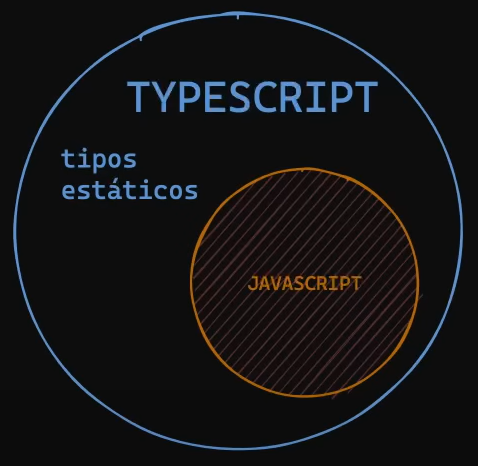
\includegraphics[width=\textwidth]{ss/1.png}
\end{figure}

TS no es un lenguaje de programación aparte como tal. TS no funciona en tiempo de ejecución, lo que llega al buscador como tal es JS. Esto es lo que el buscador recibiría de TS (\ref{tab:1}):
\begin{table}[H]
    \centering
    \caption{Código JS generado de TS}
    \label{tab:1}
    \begin{tabular}{|m{7cm}|m{7cm}|}
        \hline
        \textbf{Buscador (JS)} & \textbf{Servidor (TS)} \\
        \hline
        \parbox{7cm}{"use strict"; \\ const nombre = 'Miguel'} & const nombre = 'Miguel' \\
        \hline
    \end{tabular}
\end{table}


\subsection{¿Porqué aprenderlo?}

\begin{itemize}
    \item Por popularidad.
    \item Los tipos de datos.
    \item Mayor control sobre los resultados de funciones según los parámetros pasados.
\end{itemize}

El siguiente código muestra la clara diferencia con respecto a los tipos de datos entre TS y JS:
\begin{table}[H]
    \centering
    \caption{Aplicación de TS a código básico de JS}
    \label{tab:2}
    \begin{tabular}{|m{4cm}|m{6cm}|m{4cm}|}
        \hline
        \textbf{Lenguaje} & \textbf{Código} & \textbf{Resultado} \\
        \hline
        JS & \parbox{6cm}{function suma(a, b) \{ \\ return a + b \\ \}} & \parbox{4cm}{suma(4, 'hola') \\ '4hola'} \\
        \hline
        TS & \parbox{6cm}{function suma(a, b) \{ \\ return a + b \\ \}} & Error \\
        \hline
    \end{tabular}
\end{table}

El código de JS te permite hacer la suma de dos tipos (siempre y cuando se pueda) pero no sabes a ciencia exacta qué tipos de datos puede llegar a ingresar el usuario, haciendo vulnerable el código a cosas que no se pueden predecir. Con TS en cambio, le dices que tipo esperas en una función y qué tipo regresará, controlando los las entradas y salidas. El código de JS en TS anterior muestra un error porque no se le indica a TS el tipo de los parámetros de la función \textbf{suma}.



\section{¿Qué es la inferencia?}

La inferencia de TS se refiere a que el propio TS lee el código que estamos desarrollando e infiere (supone) el tipo de dato de las variables, funciones u objetos que estamos creando, si tenemos estos dos ejemplos:
\begin{lstlisting}
let mascota = 'mia';

const persona = {
    name = 'juan',
    age = 30
}
\end{lstlisting}

TS infiere que la variable \textit{mascota} es de tipo string por el valor contenido en esa variable, infiere que los atributos \textit{persona.name} y \textit{persona.age} son de tipo string y number, se le puede decir explícitamente el tipo, pero TS tiene esta cualidad de que infiere los tipos de las cosas. La manera de asignar un tipo a una variable, objeto o función es la siguiente 
\begin{lstlisting}
let booleano: boolean = true;
let cadena: string = 'hola';
let numero: number = 5;
let nulo: null = null;
let indefinido: undefined;
let cualquiera: any;
let desconocido: unknown;
\end{lstlisting}

Los tipos de datos básicos de JS son las cadenas (string), números (number), booleanos (boolean), null y undefined. Se utiliza el nombre de la variable, dos puntos y el tipo esperado, lo mismo para las propiedades de objetos, el valor de retorno de una función y las variables. Si se utiliza el método \textbf{typeof} con las variables tipo \textit{any} y \textit{unknown} lo que se regresará es el valor undefined.

Se recomienda ESCRIBIR LA MENOR CANTIDAD DE TIPOS DE DATOS en las variables, objetos o funciones, de eso se tiene que encargar TS. Se recomienda principalmente en variables u objetos que utilicen los tipos sencillos que se mencionaron anteriormente, para cosas más pesadas, como objetos de dependencias internas y externas, conexiones a bases de datos y otras cosas, es preferible especificar el tipo.


\subsection{Inferencia con las funciones y sus parámetros}

Por lo general, TS si logra inferir el tipo de los parámetros de una función, incluso el tipo del retorno de la función, en cualquier caso se recomienda revisar qué es lo que dice el IDE, editor de texto o TS con respecto al tipo inferido, si es any, asignar el tipo que realmente se espera, esto con el fin de seguir la regla de escribir la menor cantidad de tipos posibles.

En caso de mandar un objeto como parámetro a una función sin haberlo declarado antes también se recibe este objeto como any en todas sus propiedades, por lo que es recomendable tiparlo para evitar conflictos. Se puede tipar de dos maneras:
\begin{lstlisting}
// opcion 2
function saludar({name, age}: {name: string, age: number}) {
    console.log(`Hola ${name} y tu edad es ${age}.`);
}

// opcion 2
function saludar(persona: {name: string, age: number}) {
    const { name, age } = persona
    console.log(`Hola ${name}, y tu edad es ${age}.`);
}
\end{lstlisting}

Con la segunda manera tendríamos que hacer \textit{destructuring} del objeto para acceder a sus propiedades.


\subsection{Inferencia en funciones como parámetro}

Como sabemos, las funciones en JS se pueden usar como parámetro dentro de otra función, y el tipado tiene que ver con esta forma de trabajar los parámetros. Pongamos el siguiente ejemplo:
\begin{lstlisting}
const sayHiFromFunction = (fn) => {
    return fn('Miguel')
}

sayHiFromFunction((name) => {
    console.log(`Hola ${name}$`)
})
\end{lstlisting}

TS tendría el problema de no poder identificar el tipo del parámetro \textbf{fn} y \textbf{name}, sabe que es una función parámetro pero no sabe qué tipo es, por lo que le asignará un tipo \textbf{any}, y como se ha dicho anteriormente, debemos evitar usar este tipo lo más que se pueda.

Hay una especia de tipo llamada Function, la cual le indica a JS que una función es una función como tal de manera muy general, es como asignarle el tipo Function a una función; utilizar este tipo para tipar una función es incorrecto, ya que si, una función será un tipo función, pero para los fines de lo que regresa o no nuestra función es incorrecto, las funciones siempre se deben de tipar según el tipo que vayan a retornar (si no retornan nada, se tipan como \textbf{void})

Solucionando el ejemplo anterior, quedaría de la siguiente manera:
\begin{lstlisting}
const sayHiFromFunction = (fn: (name: string) => void) => {
    return fn('Miguel')
}

const sayHi = (name: string) => {
    console.log(`Hola ${name}$`)
}

sayHiFromFunction(sayHi)
\end{lstlisting}

La función sayHi (que antes estaba insertada dentro de los parámetros de sayHiFromFunction) no regresa nada, pero tiene un parámetro string, por lo que sayHiFromFunction se tipa como que tiene una función parámetro que a la vez tiene un parámetro (\textit{fn: (name: string)}) y no retorna nada (\textit{fn: (name: string) =$>$ void}).


\subsection{Inferencia en funciones anónimas}

Por lo general, TS si logra inferir correctamente el tipo de una función anónima, pondremos de ejemplo lo siguiente:
\begin{lstlisting}
const avengers = ['spiderman', 'hulk', 'avengers']

avengers.forEach(function (avenger) {
    console.log(avenger.toUpperCase())
})    
\end{lstlisting}

El arreglo \textbf{avengers} es de tipo string por la inferencia de TS, al usar un método de arreglos (forEach) el cual solicita una función que realice una acción, TS infiere que la función a utilizar también es string, esto por el tipo del arreglo.



\section{Asignando tipos de datos}


\subsection{Funciones regulares}

Para tipar una función regular (que utiliza la palabra reservada function), se hace de la siguiente manera:
\begin{lstlisting}
function sumar(a: number, b: number) : number {
    return a + b;
}
\end{lstlisting}


\subsection{Funciones arrow}

Para tipar una función arrow, se hace de la siguiente manera:
\begin{lstlisting}
const sumar = (a: number, b: number): number => {
    return a + b
}
\end{lstlisting}


\subsection{Funciones anónimas}

Recordemos que una función anónima es aquella que son aquellas que no han sido declaradas con un nombre, generalmente las encontramos en las funciones utilizadas por arreglos (map o filter por ejemplo). Se tipan de la siguiente manera:
\begin{lstlisting}
const arreglo = ['a', 'b', 'c']

arreglo.forEach((item: string) => {
    console.log(item)
})
\end{lstlisting}


\subsection{Tipos especiales de TS}

El tipo \textbf{any} se utiliza para, literalmente, decirle a TS que la variable u objeto puede ser de cualquier tipo, por lo cual, el lenguaje deja de recomendarnos métodos especiales para los tipos existente. Dicho en otras palabras, con any se ignora completamente el tipado que ofrece TS. Se recomienda usar lo menos posible este tipo.

El tipo \textbf{unknown} se utiliza cuando uno no sabe el tipo de dato que esperar de una variable, asignando este tipo a una variable TS no recomienda métodos especiales para tipos porque no sabe el tipo de la variable u objeto.

El tipo \textbf{never} se utiliza cuando se tiene una función donde se tiene una certeza del 100\% de que esta no devolverá ningún tipo de variable. Generalmente se utiliza en funciones que lanzan un mensaje de error como la siguiente:
\begin{lstlisting}
function throwError(message: string): never {
    throw new Error(message);
}
\end{lstlisting}

Otro ejemplo un poco más claro sobre la aparición del tipo never:
\begin{lstlisting}
function fn(x: string | number) {
    if(typeof x == 'string') {
        // type string.
        // do something.
    }
    else if(typeof x == 'number') {
        // type number.
        // do something.
    }
    else {
        x // type never.
    }
}
\end{lstlisting}



\section{Tipos propios}


\subsection{Types alias}

Podemos crear alguna especie de tipo de dato para asignárselo a objetos y que estos tengan un tipo de dato en lugar de que sean simplemente objetos sin tipo; podría decirse que es como crear una clase, la clase es una clase como tal y tiene propiedades y métodos dentro de ella que son de cierto tipo, luego podemos crear objetos de la clase y estos objetos son del tipo de la clase. Visto en C\# se ve así:
\begin{lstlisting}
// se crea la clase.
class Persona
{
    // metodos y atributos de cierto tipo.
    public string Nombre;
    public int Edad;
}

// se crea el objeto.
Persona persona = new Persona();
\end{lstlisting}

Con los type alias sería así:
\begin{lstlisting}
// se crea el alias.
type Persona = {
    Nombre: string
    Edad: number
}

let persona: Persona = {
    Nombre: 'thor',
    Edad: 1500
}
\end{lstlisting}

Ahora el objeto tiene un tipo definido.


\subsection{Union types}

Podemos crear un tipo el cual solamente pueda recibir ciertos valores o cierto tipo de dato, para el primer caso, es como si tuviéramos un if o switch donde, según el valor recibido, se le asigne otro valor a una variable, para el segundo caso, podemos decirle TS que la variable que estamos declarando puede ser un número o una cadena, una cadena o un booleano, un número o booleano, etc.

Veamos ambos casos
\begin{lstlisting}
type heroLevel = 'low' | 'medium' | 'high'

var a : number | string

var hero1 : heroLevel = 'extreme' // error.
var hero2 : heroLevel = 'low' // correcto.
a = true // error.
a = 2 // correcto.
\end{lstlisting}

Incluso se puede optar por un tipo o un valor concreto:
\begin{lstlisting}
var b : number | 'hola'
\end{lstlisting}


\subsection{Templates union types}

Podemos crear un tipo que esté constituido de otros tipos según un patrón o las necesidades que tengamos, por ejemplo, hablando de los Ids, podemos crear un formato de Id donde aparezcan 3 cadenas separadas por un guión:
\begin{lstlisting}
type PersonaId = `${string}-${string}-${string}`
\end{lstlisting}

Este tipo ahora se puede usar dentro de objetos u otros tipos:
\begin{lstlisting}
type Persona = {
    Id: PersonaId
    Nombre: string
    Edad: number
}
\end{lstlisting}


\subsection{Propiedades opcionales}

Como vimos anteriormente, podemos crear types alias, los cuales tienen propiedades de cierto tipo, podemos hacer que algunas de estas propiedades no sean obligatorias al momento de aplicar estos alias a objetos mediante el símbolo ?:
\begin{lstlisting}
type Persona = {
    Id?: PersonaId
    Nombre: string
    Edad: number
}
\end{lstlisting}

Ahora, cuando se cree un objeto tipo Persona, no será obligatorio rellenar la propiedad Id.


\subsection{Intersection types}

Otra cosa muy interesante que se puede hacer es poder combinar tipos diferentes en uno solo, armando así un nuevo tipo constituido de otros, veamos este ejemplo: tenemos un tipo HeroBasicInfo, el cual contiene dos atributos obligatorios que son el nombre y edad de un héroe, también tenemos HeroProperties, el cual tiene otros atributos no obligatorios del héroe, como sería su status y escala de poder:

\begin{lstlisting}
type heroLevel = 'low' | 'medium' | 'high'

type HeroBasicInfo = {
    nombre: string,
    edad: number
}

type HeroProperties = {
    isActive?: boolean,
    powerScale?: heroLevel
}
\end{lstlisting}

HeroLevel es un complemento visto en uno de los ejemplos anteriores. Si queremos combinar estos dos tipos se hace de la siguiente manera:
\begin{lstlisting}
type Hero = HeroBasicInfo & HeroProperties;

let hero3 = {
    name: 'spiderman',
    age: 30
}
\end{lstlisting}

De esta manera, tenemos los atributos de ambos tipos en uno solo, así el tipo puede recibir menor cantidad de atributos y aligerar la carga de trabajo.


\subsection{Types indexing}

En caso de que tengamos un tipo con un objeto como atributo, al momento de querer acceder a este objeto y querer asignar valores en una variable o constante, podemos utilizar el type indexing para lograr este cometido:
\begin{lstlisting}
type HeroProperties = {
    isActive: boolean,
    address: {
        planet: string,
        city: string
    }
}

const addressHero: HeroProperties['address'] = {
    planet: 'Tierra',
    city: 'Madrid'
}
\end{lstlisting}

Vemos que se crea el tipo HeroProperties el cual tiene un objeto llamado 'address' dentro, al crear una variable tipo HeroProperties, podemos acceder al objeto dentro del tipo solamente utilizando los corchetes con el nombre del objeto que deseamos utilizar, como se ve en la constante addressHero.


\subsection{Types de valores y funciones}

Si declaramos un objeto con ciertos atributos de x tipo, podemos crear un tipo que sea igual a este objeto:
\begin{lstlisting}
const address = {
    planet: 'Tierra',
    city: 'Madrid'
}

type Address = typeof address
\end{lstlisting}

Esto se puede transportar a lo que regresa un función:
\begin{lstlisting}
function createAddress() {
    return {
        planet: 'Tierra',
        city: 'Madrid'
    }
}

type Address = ReturnType<typeof createAddress>
\end{lstlisting}

ReturnType recupera el tipo de alguna función que le pases, en este caso recupera el tipo del objeto que regresa la función createAddress, el cual es un objeto con dos atributos tipo string.
